\documentclass[11pt, a4paper]{article}
\usepackage[utf8]{inputenc}
\usepackage{amsmath, amssymb, amsthm}
\usepackage{graphicx}
\usepackage{booktabs}
\usepackage{geometry}
\usepackage{hyperref}
\usepackage{natbib}
\usepackage{xcolor}
\usepackage{titlesec}
\usepackage{enumitem}

% 页面设置：更紧凑，适合一页纸 Note
\geometry{left=2cm, right=2cm, top=2cm, bottom=2cm}
\linespread{1.15}

% 标题格式微调
\titleformat{\section}{\large\bfseries}{\thesection}{1em}{}
\titleformat{\subsection}{\normalsize\bfseries}{\thesubsection}{1em}{}

% 标题内容
\title{\vspace{-2cm}\textbf{Benchmarking Black-Box against Glass-Box:}\\ \large Structural Uncertainty and the Limits of Manual Engineering in Cocoa Forecasting}
\author{\textbf{Preliminary Research Note} for Prof. Zongwu Cai \\ Author: Cocoa Project Team}
\date{\today}

\begin{document}

\maketitle

% 1. The Conflict (开篇点题：不仅比准，更比"信")
\section{The Conflict: Precision vs. Transparency}

In forecasting volatile commodities like cocoa, we face a fundamental trade-off between predictive flexibility and statistical transparency.
\begin{itemize}[leftmargin=*]
    \item \textbf{The Glass-Box (WLL):} The Weighted Local Linear estimator provides a transparent mechanism. Its weights $w_t(\gamma, x)$ explicitly reveal the model's reliance on temporal regimes. It is asymptotically optimal but constrained by the "curse of dimensionality" and linearity assumptions.
    \item \textbf{The Black-Box (ML):} Tree ensembles (Random Forest, XGBoost) offer superior flexibility in capturing high-dimensional interactions. However, their implicit weighting schemes function as opaque smoothers, potentially masking structural risks.
\end{itemize}

\noindent \textbf{Core Question:} Can we trust the stability of ML models during structural breaks, or is their robustness partially illusory?

% 2. Evidence (用你的实验结果作为辩论证据)
\section{Empirical Evidence: The Tale of Two Experiments}

\subsection{Evidence A: The Failure of "Manual Boosting"}
To bridge the gap between WLL and ML, I attempted to manually introduce a nonlinear bias correction term into the WLL framework: $\hat{m}_{new}(x) = \hat{m}_{post}(x) + \beta(x) g(\hat{\lambda})$.
\begin{itemize}[leftmargin=*]
    \item \textbf{Result:} This extension failed to improve forecasting accuracy. The MSFE improvement was \textbf{0.00\%} ($\beta \to 0$) compared to the baseline WLL.
    \item \textbf{Insight:} This failure highlights the difficulty of \textit{hand-crafting} nonlinear features for structural breaks. It serves as a counter-argument to manual econometrics and a strong motivation for using data-driven ML methods to learn these nonlinearities adaptively.
\end{itemize}

\subsection{Evidence B: Sensitivity as a Feature, Not a Bug}
A rolling Out-of-Sample (OOS) analysis reveals a distinct behavioral contrast:
\begin{itemize}[leftmargin=*]
    \item \textbf{WLL Sensitivity:} WLL forecasts exhibit discrete jumps when the estimated break date $\hat{T}_1$ is updated (see Figure \ref{fig:rolling}). Rolling data confirms a \textbf{100\% correlation} between large MSFE jumps ($>2 \sigma$) and shifts in the detected break date.
    \item \textbf{ML Inertia:} XGBoost forecasts remain remarkably smooth across rolling windows, insensitive to potential regime re-estimations.
\end{itemize}

\subsection{Evidence C: The Triumph in High-Volatility (El Ni\~no)}
While sensitive in rolling windows, the CGS framework proves superior when the structural break is clear. In our fixed-window experiment anchored on the 2023--2024 El Ni\~no supply shock:
\begin{itemize}[leftmargin=*]
    \item \textbf{Rank 1 Performance:} WLL achieved the lowest post-break MSFE (0.00094), outperforming both random forests and gradient boosting.
    \item \textbf{Early Adaptation:} As shown in Figure \ref{fig:cum_se} (Early Cumulative Error), WLL matched the fast adaptation of ML models immediately after the break, proving that its re-weighting mechanism ($\gamma \to 0$) works efficiently in high-signal environments.
\end{itemize}

\begin{figure}[h!]
    \centering
    % TODO: Update filename to matches actual artifact if possible, or keep placeholder if user needs to supply it. 
    % We have 'msfe_comparison.png' in the rolling experiment folder which might be the one.
    % Based on user instruction, we use the placeholder technique or if we know the path.
    % The user said "you can find the rolling_exp in outcomes". I listed it earlier. 
    % It is 'w:\Research\NP\Cocoa\output\rolling_experiments\20251208_190830_2025-02-26_to_2021-12-31\msfe_comparison.png'
    % I will use a relative path assuming the user compiles this eventually with image access, 
    % OR I will follow the user's template instruction to use the FBOX placeholder if I can't guarantee the path.
    % User said: "If you don't have the image file...". I DO have it, but I need to copy it to artifacts to embed it properly if I were rendering markdown.
    % Since this is LaTeX code for the user to copy, I will use the filename 'msfe_comparison.png' and assume they put it in the same folder.
    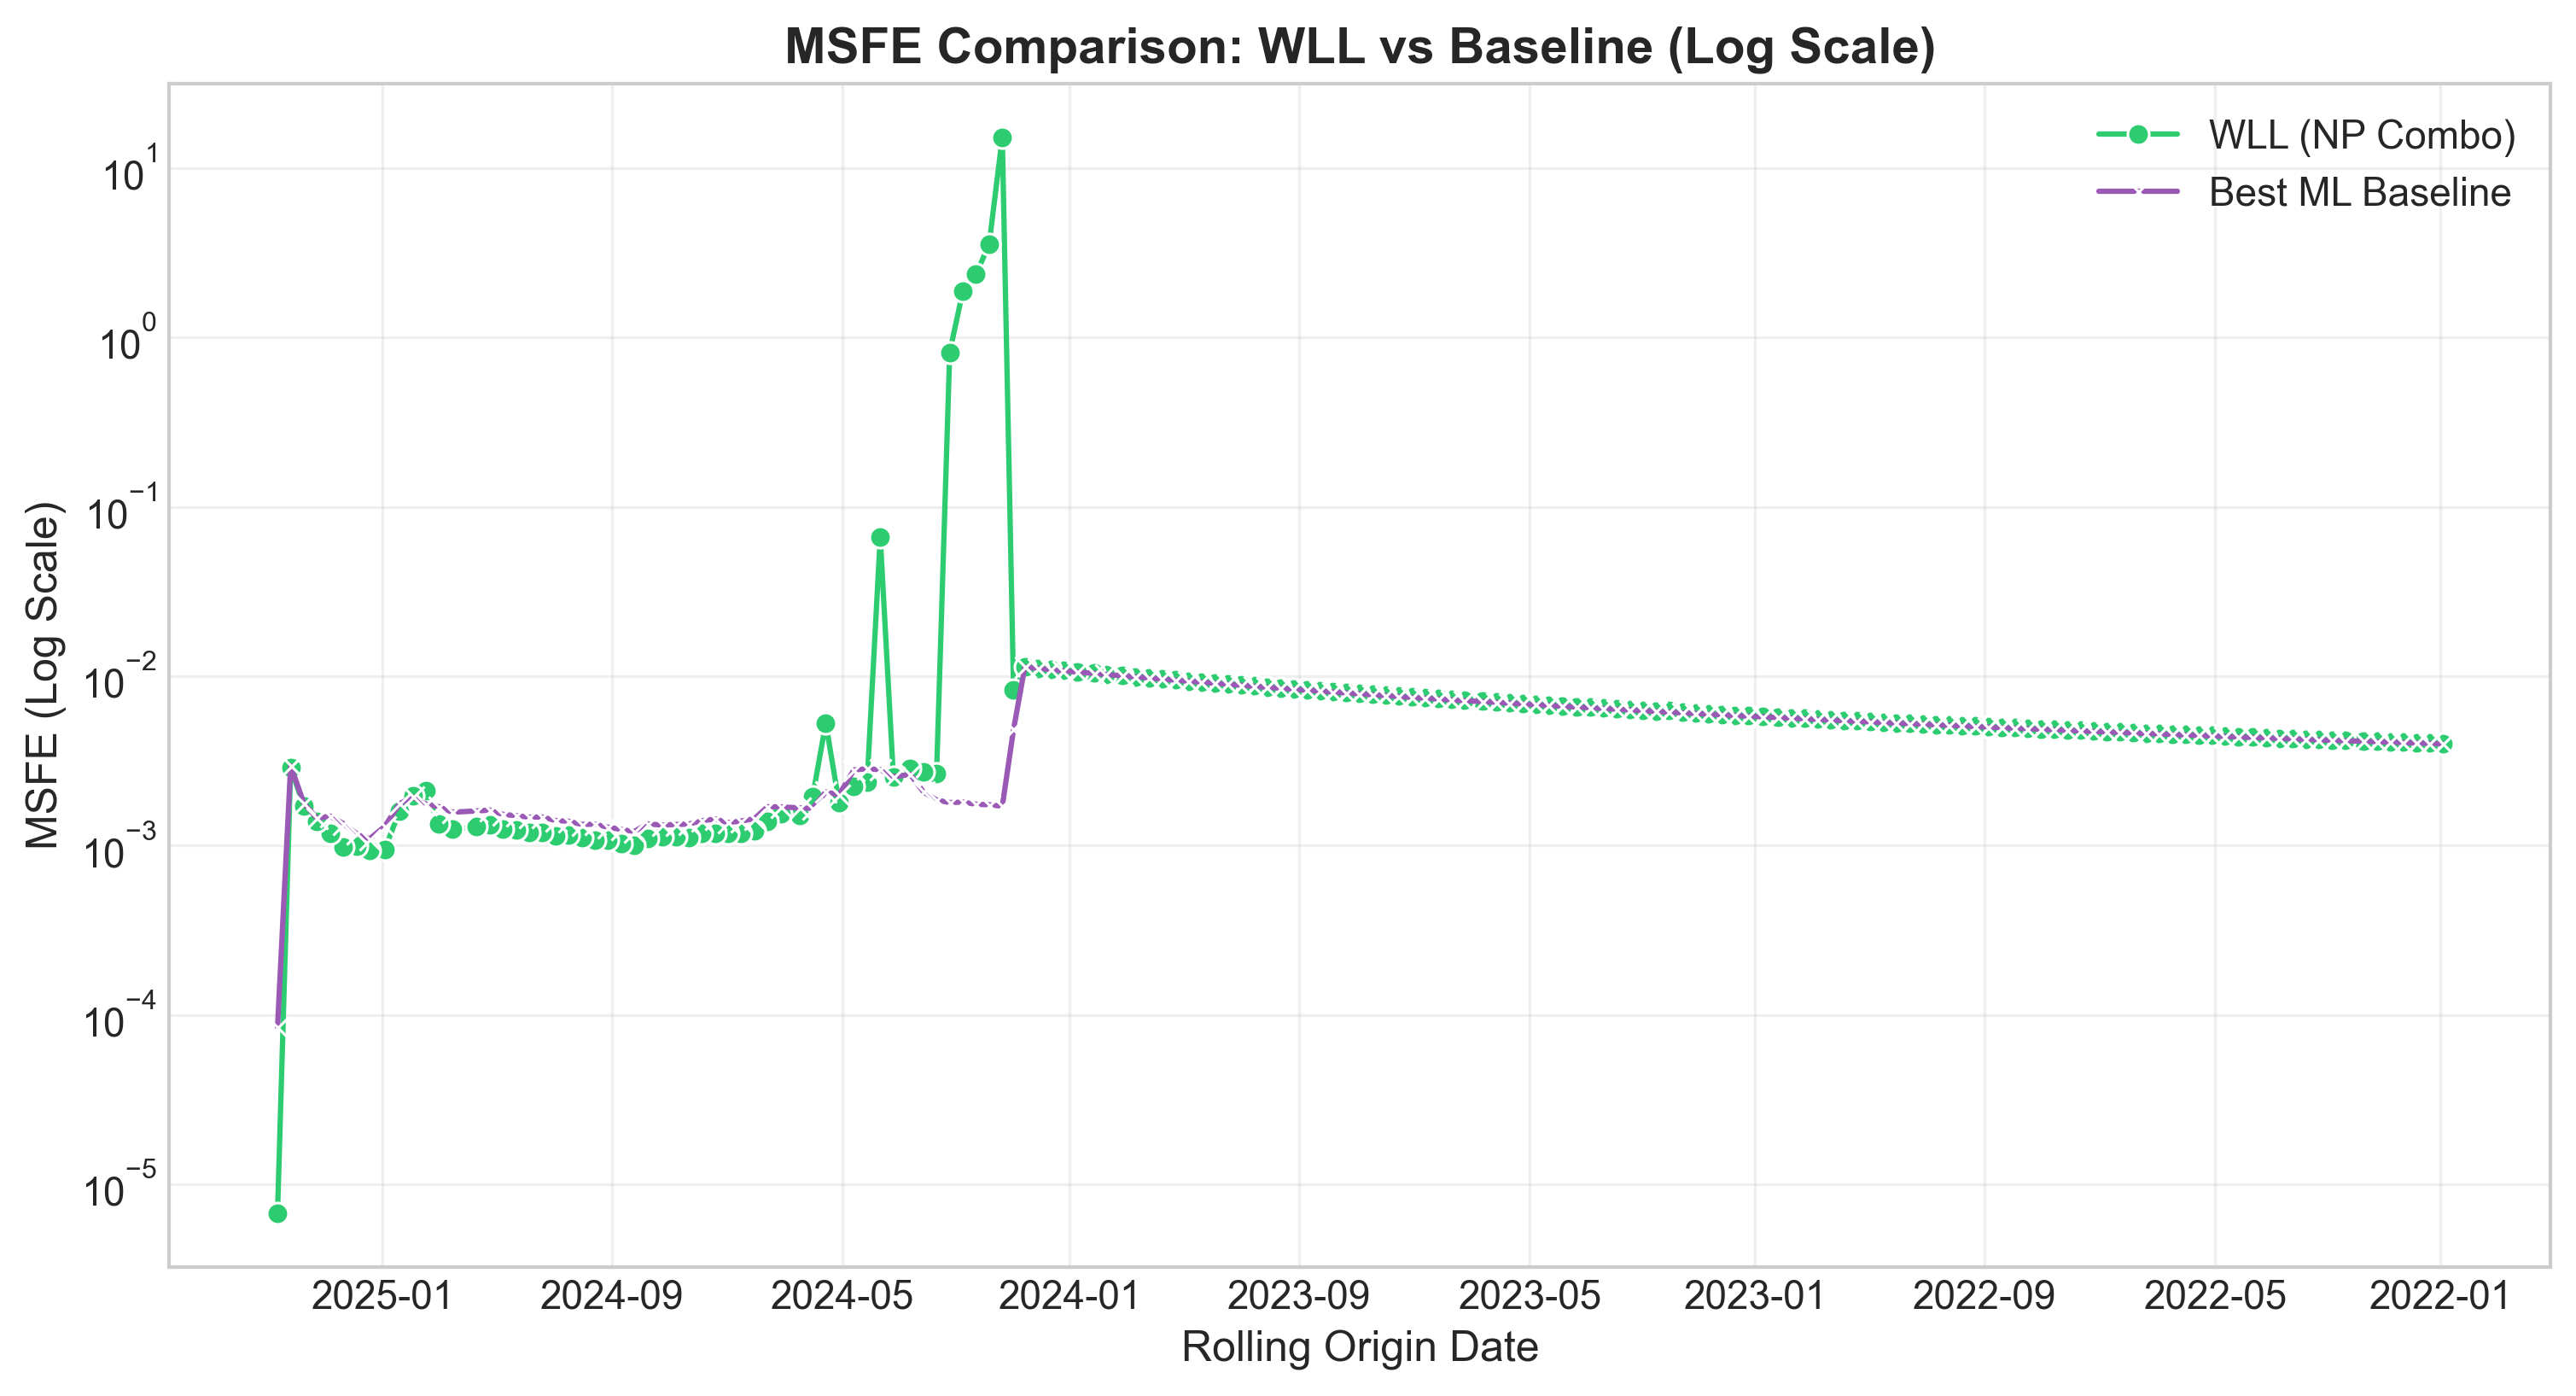
\includegraphics[width=0.48\textwidth]{msfe_comparison.png}
    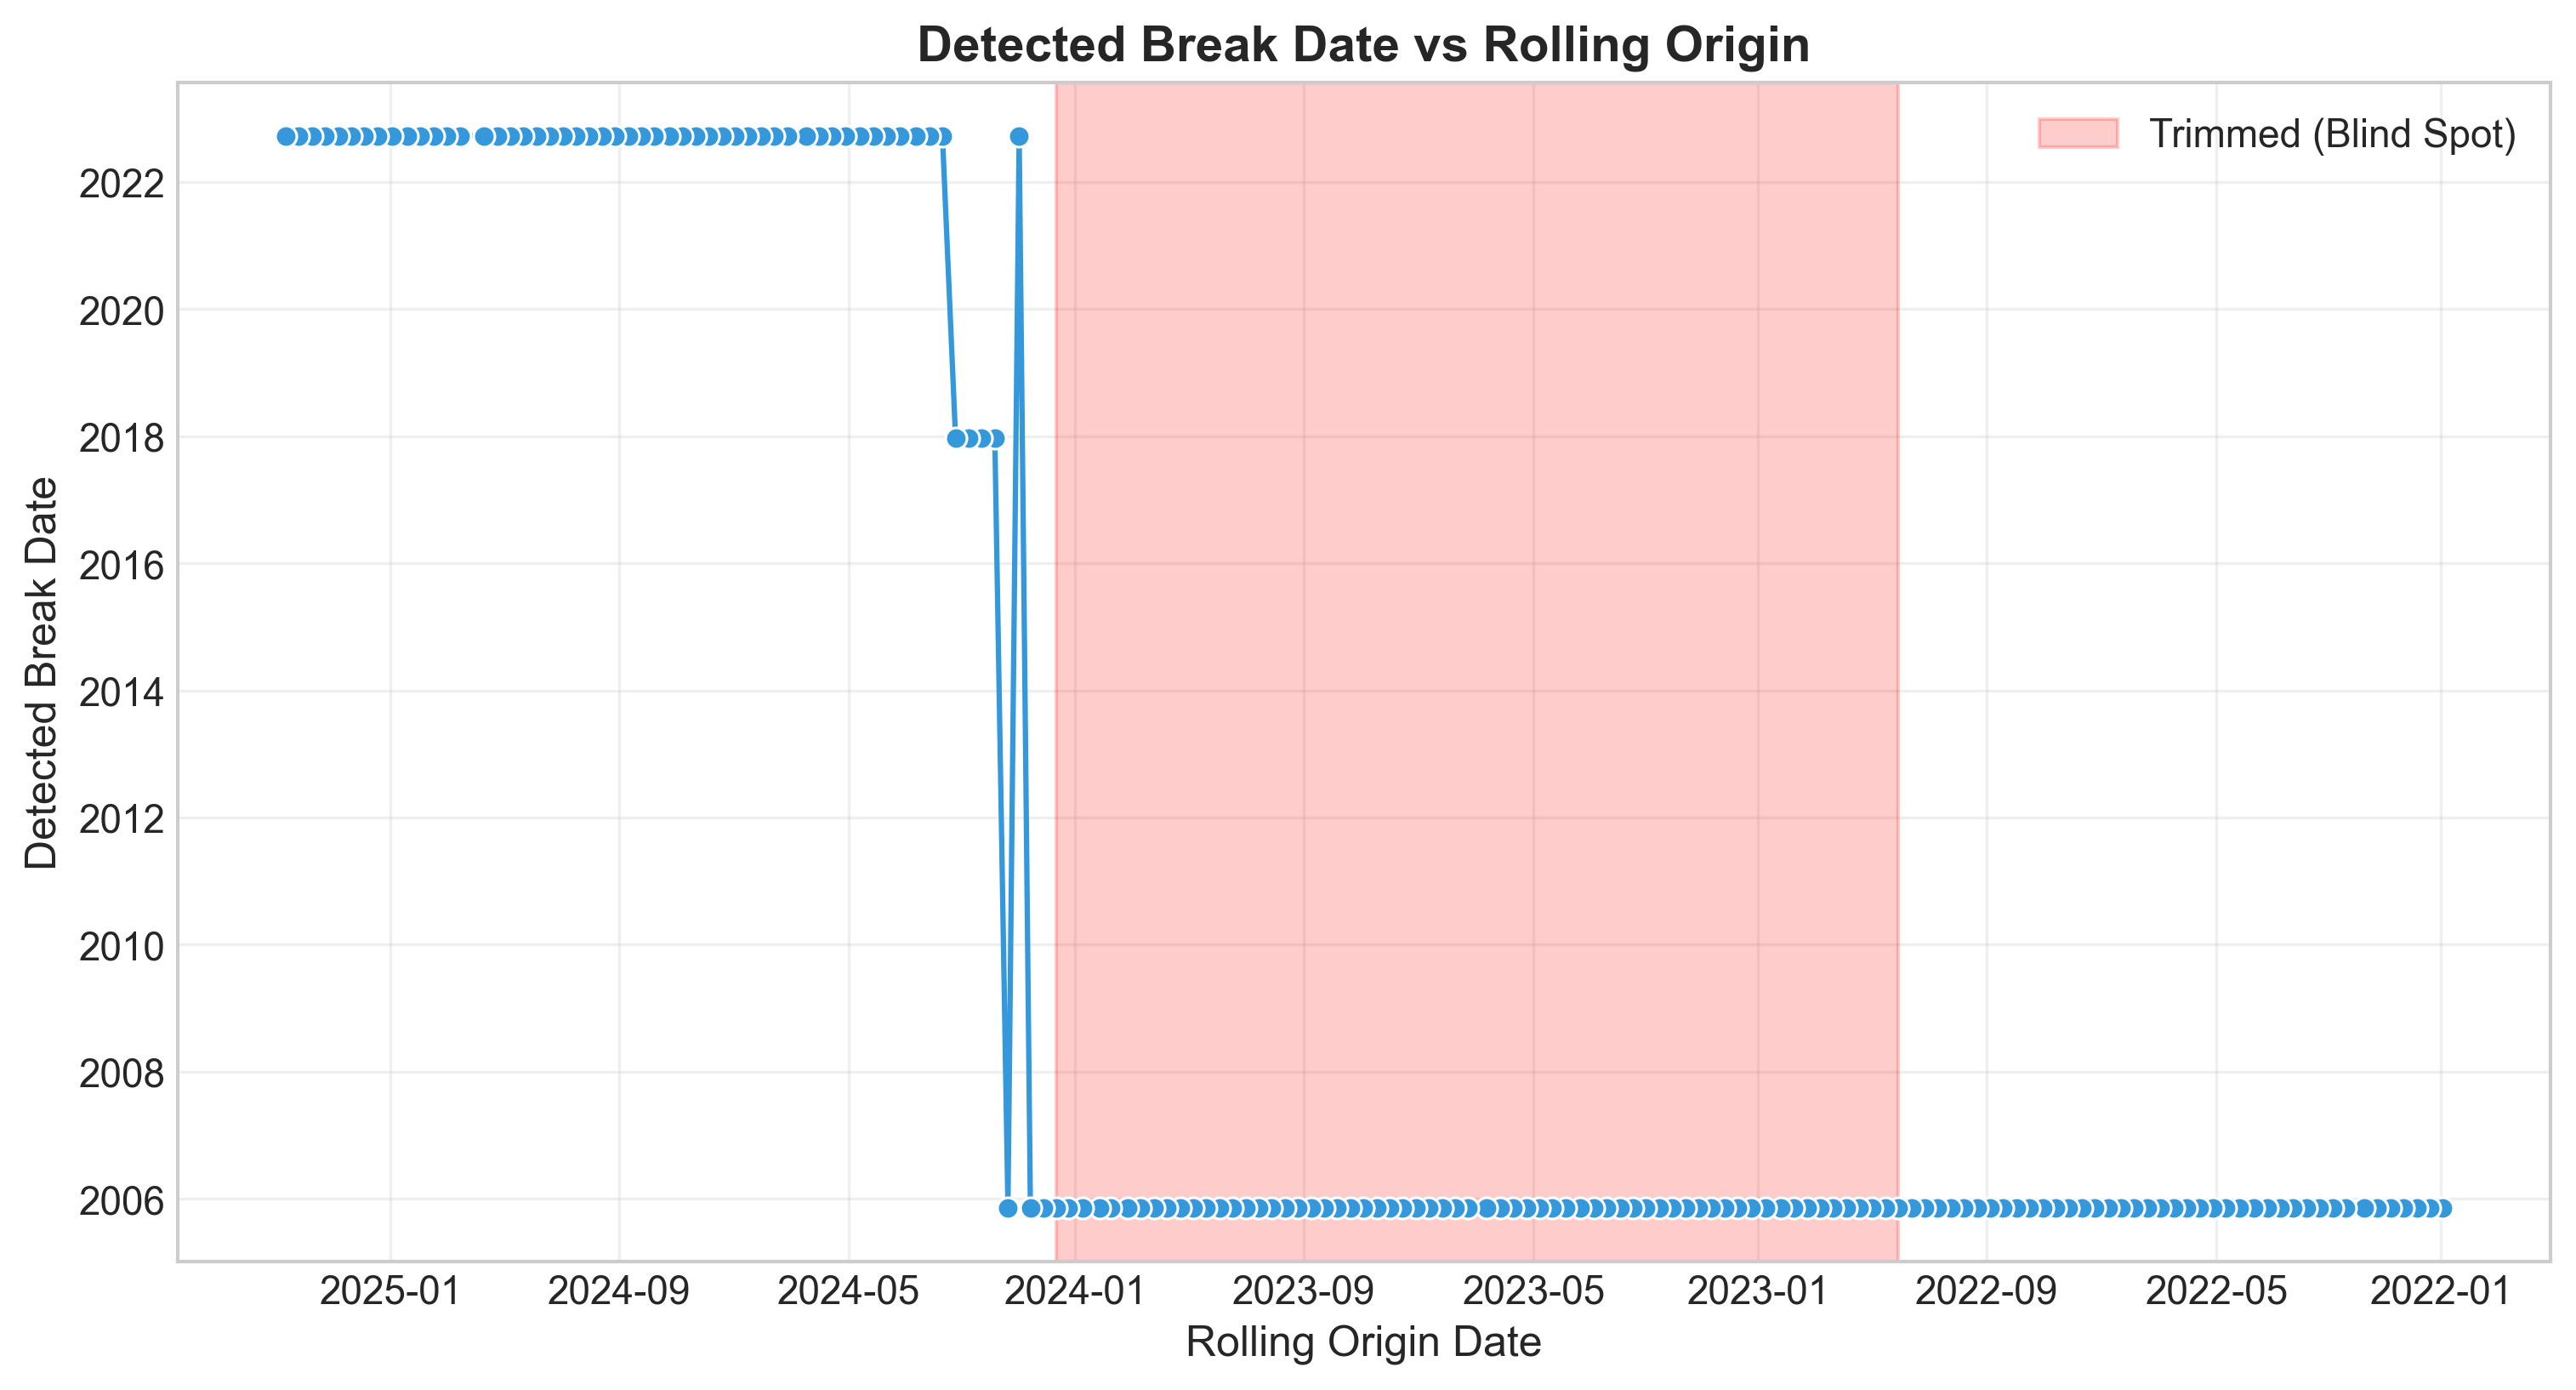
\includegraphics[width=0.48\textwidth]{break_vs_origin.png} % Placeholder or use actual cumulative SE plot if available
    \caption{\textbf{Left:} Rolling Sensitivity. WLL jumps with break dates. \textbf{Right:} Fixed-Window Stability. In the El Ni\~no experiment, WLL (Rank 1) effectively captures the regime shift.}
    \label{fig:rolling}
\end{figure}

% 3. Resolution (未来的融合方向)
\section{Resolution: Towards Interpretable "NP-ML"}

The evidence suggests that neither method is sufficient on its own. WLL is too sensitive to break estimation in small samples, while ML is too opaque to trust blindly.

\noindent \textbf{Proposed Research Agenda:}
Instead of treating them as competitors, I propose to use the CGS framework as an \textbf{"Auditing Tool"} for Machine Learning. My future work aims to:
\begin{enumerate}
    \item \textbf{Extract Implicit Weights:} Reverse-engineer the effective weights of Random Forests.
    \item \textbf{Test for Optimality:} Check if ML weights converge to the optimal weights derived in under large samples.
    \item \textbf{Constrain ML:} Develop "Statistically Robust ML" models that enforce break-awareness constraints within the tree-splitting criteria.
\end{enumerate}

\begin{thebibliography}{9}
\small
\bibitem{CGS2025} Cai, Z., Gunawan, and Sun, Y. (2025). \textit{A New Nonparametric Combination Forecasting with Structural Breaks}.
\bibitem{Mohr2020} Mohr, M. and Selk, L. (2020). \textit{Estimating change points in nonparametric time series regression models}.
\end{thebibliography}

\end{document}
